% Plot Tiefpass
% Minimalistisch (sketch-like for beamer presentation)
% Phasengang
% plots with same width for vertical alignment:
%   plot_tiefpass_mini_ampli_lin_samesize.tex
%   plot_tiefpass_mini_phase_lin_samesize.tex
%   plot_hochpass_mini_ampli_lin_samesize.tex
%   plot_hochpass_mini_phase_lin_samesize.tex
% TODO: Alignment via invisible boundbox
\def\ttau{0.01}%                % Zeitkonstante tau = 0.01 s
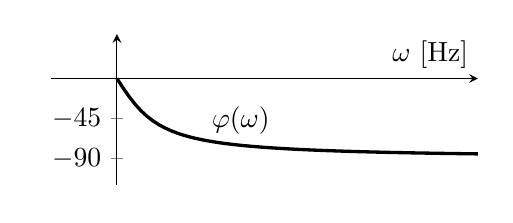
\begin{tikzpicture}%
    % invisible boundbox
    \draw[draw=none](-0.3,-0.125) rectangle (+5.5,+2); % bbox % set draw=black (debug) or draw=none (final)
\begin{axis}[%
    xlabel={$\omega\ [\mathrm{Hz}]$},
    xmin=-200, xmax=1100,       % alignment solution with x-axis (bigger than y-labels):
    domain=0:1100, 
    ymin=-120, ymax=50,
    samples=61,
    axis x line=center,
    axis y line=center,
    width=7cm,
    height=3.5cm,
    ytick={0,-45,-90},
    yticklabels={$0\degree$,$-45\degree$,$-90\degree$},
    xtick=\empty,
]   % varphi(omega) = arctan(-omega*tau)
    \addplot[mark=none,very thick,]   {atan(-x*\ttau)}  node [pos=0.35,anchor=south] {$\varphi(\omega)$};% plot + plotlabel
    %\addplot[mark=none] coordinates{(950,-30)} node {$\omega\ \left[\mathrm{Hz}\right]$};% x-axis label
\end{axis}%
\end{tikzpicture}% Keine Leerzeichen danach!